\newcommand{\titulus}{\nomenFesti{Dominica III post Pascha.}
\celebratio{Semiduplex.}}
\newcommand{\capitulumLaudes}{\pars{Capitulum.} \scriptura{1 Petr. 2, 11}

\grechangedim{interwordspacetext}{0.12 cm plus 0.15 cm minus 0.05 cm}{scalable}%
\cuminitiali{}{temporalia/capitulum-CarissimiObsecro.gtex}
\grechangedim{interwordspacetext}{0.22 cm plus 0.15 cm minus 0.05 cm}{scalable}}
\newcommand{\magnificati}{\pars{Canticum B. Mariæ V.} \scriptura{Io. 16, 17; \textbf{H243}}

\vspace{-6mm}

{
\grechangedim{interwordspacetext}{0.18 cm plus 0.15 cm minus 0.05 cm}{scalable}%
\antiphona{VI F}{temporalia/ant-modicumetnon.gtex}
\grechangedim{interwordspacetext}{0.22 cm plus 0.15 cm minus 0.05 cm}{scalable}%
}

%\trAntIMagnificat

\vspace{-4mm}

\scriptura{Lc. 1, 46-55}

\cantusSineNeumas
\initiumpsalmi{temporalia/magnificat-initium-visoll-F.gtex}

%\vspace{-7mm}

%\psalmusEtTranslatioT{temporalia/magnificat-V-comb.tex}{10.2cm}
\input{temporalia/magnificat-V.tex} \Abardot{}}
\newcommand{\lectioi}{\pars{Lectio I.} \scriptura{Ap. 1, 1-6}

\noindent Incipit liber Apocalýpsis beáti Ioánnis Apóstoli.

\noindent Apocalýpsis Iesu Christi, quam dedit illi Deus palam fácere servis suis, quæ opórtet fíeri cito: et significávit, mittens per ángelum suum servo suo Ioánni, qui testimónium perhíbuit verbo Dei, et testimónium Iesu Christi, quæcúmque vidit. Beátus qui legit, et audit verba prophetíæ huius, et servat ea, quæ in ea scripta sunt: tempus enim prope est. Ioánnes septem ecclésiis, quæ sunt in Asia. Grátia vobis, et pax ab eo, qui est, et qui erat, et qui ventúrus est: et a septem spirítibus qui in conspéctu throni eius sunt: et a Iesu Christo, qui est testis fidélis, primogénitus mortuórum, et princeps regum terræ, qui diléxit nos, et lavit nos a peccátis nostris in sánguine suo, et fecit nos regnum, et sacerdótes Deo et Patri suo: ipsi glória et impérium in sǽcula sæculórum. Amen.}
\newcommand{\responsoriumi}{\pars{Responsorium 1.} \scriptura{\Rbardot{} Ap. 5, 9; \Vbardot{} ibid. 5, 10; \textbf{H247}}

\vspace{-5mm}

\responsorium{VII}{temporalia/resp-dignusesdomine-sinedox.gtex}{}}
\newcommand{\lectioii}{\pars{Lectio II.} \scriptura{Ap. 1, 7-11}

\noindent Ecce venit cum núbibus, et vidébit eum omnis óculus, et qui eum pupugérunt. Et plangent se super eum omnes tribus terræ. Etiam: amen. Ego sum alpha et ómega, princípium et finis, dicit Dóminus Deus: qui est, et qui erat, et qui ventúrus est, omnípotens. Ego Ioánnes frater vester, et párticeps in tribulatióne, et regno, et patiéntia in Christo Iesu: fui in ínsula, quæ appellátur Patmos, propter verbum Dei, et testimónium Iesu: fui in spíritu in domínica die, et audívi post me vocem magnam tamquam tubæ, dicéntis: Quod vides, scribe in libro: et mitte septem ecclésiis, quæ sunt in Asia, Epheso, et Smyrnæ, et Pérgamo, et Thyatíræ, et Sardis, et Philadelphíæ, et Laodicíæ.}
\newcommand{\responsoriumii}{\pars{Responsorium 2.} \scriptura{\Rbardot{} Eccli. 24, 23.26; \Vbardot{} ibid. 24, 25; \textbf{H247}}

\vspace{-5mm}

\responsorium{III}{temporalia/resp-egosicutvitis-sinedox.gtex}{}}
\newcommand{\lectioiii}{\pars{Lectio III.} \scriptura{Ap. 1, 12-19}

\noindent Et convérsus sum ut vidérem vocem, quæ loquebátur mecum: et convérsus vidi septem candelábra áurea: et in médio septem candelabrórum aureórum, símilem Fílio hóminis vestítum podére, et præcínctum ad mamíllas zona áurea: caput autem eius, et capílli erant cándidi tamquam lana alba, et tamquam nix, et óculi eius tamquam flamma ignis: et pedes eius símiles aurichálco, sicut in camíno ardénti, et vox illíus tamquam vox aquárum multárum: et habébat in déxtera sua stellas septem: et de ore eius gládius utráque parte acútus exíbat: et fácies eius sicut sol lucet in virtúte sua. Et cum vidíssem eum, cécidi ad pedes eius tamquam mórtuus. Et pósuit déxteram suam super me, dicens: Noli timére: ego sum primus, et novíssimus, et vivus, et fui mórtuus, et ecce sum vivens in sǽcula sæculórum: et hábeo claves mortis, et inférni. Scribe ergo quæ vidísti, et quæ sunt, et quæ opórtet fíeri post hæc.}
\newcommand{\responsoriumiii}{\pars{Responsorium 3.} \scriptura{\Rbardot{} Ap. 14, 2 \& Ap. 11, 15 \& Fulgentius Ruspensis (pseudo): Liber de Trinitate, cap. 6; \Vbardot{} Ap. 19, 5; \textbf{H247}}

\vspace{-5mm}

\responsorium{VII}{temporalia/resp-audivivocemincaelotamquam-cumdox.gtex}{}}
\newcommand{\lectioiv}{\pars{Lectio IV.} \scriptura{Sermo 147 de Tempore}

\noindent Sermo sancti Augustíni Epíscopi.

\noindent Diébus his sanctis resurrectióni Dómini dedicátis, quantum donánte ipso póssumus, de carnis resurrectióne tractémus. Hæc enim est fides nostra: hoc donum in Dómini nostri Iesu Christi nobis carne promíssum est, et in ipso præcéssit exémplum. Vóluit enim nobis, quod promísit in fine, non solum prænuntiáre, sed étiam demonstráre. Illi quidem qui tunc fuérunt, cum illum vidérent, et cum expavéscerent, et spíritum se vidére créderent, soliditátem córporis tenuérunt. Locútus est enim non solum verbis ad aures eórum, sed étiam spécie ad óculos eórum: parúmque erat se præbére cernéndum, nisi étiam offérret pertractándum atque palpándum.}
\newcommand{\responsoriumiv}{\pars{Responsorium 4.} \scriptura{\Rbardot{} Ap. 21, 9.2; \Vbardot{} ibid. 21, 10; \textbf{H247}}

\vspace{-5mm}

\responsorium{II}{temporalia/resp-locutusestadmeunus-sinedox.gtex}{}}
\newcommand{\lectiov}{\pars{Lectio V.}

\noindent Ait enim: Quid turbáti estis, et cogitatiónes ascéndunt in cor vestrum? Putavérunt enim se spíritum vidére. Quid turbáti estis, inquit, et cogitatiónes ascéndunt in cor vestrum? Vidéte manus meas, et pedes meos: palpáte, et vidéte: quia spíritus ossa et carnem non habet, sicut me vidétis habére. Contra istam evidéntiam disputábant hómines. Quid enim áliud fácerent hómines, qui ea, quæ sunt hóminum, sápiunt, quam sic disputáre de Deo contra Deum? Ille enim Deus est, isti hómines sunt. Sed Deus novit cogitatiónes hóminum, quóniam vanæ sunt.}
\newcommand{\responsoriumv}{\pars{Responsorium 5.} \scriptura{\Rbardot{} Ap. 14, 7; \Vbardot{} ibid. 14, 6.7; \textbf{H248}}

\vspace{-5mm}

\responsorium{I}{temporalia/resp-audivivocemincaeloangelorum-sinedox.gtex}{}}
\newcommand{\lectiovi}{\pars{Lectio VI.}

\noindent In hómine carnáli tota régula intelligéndi est consuetúdo cernéndi. Quod solent vidére, credunt: quod non solent, non credunt. Præter consuetúdinem facit Deus mirácula, quia Deus est. Maióra quidem mirácula sunt, tot quotídie hómines nasci, qui non erant, quam paucos resurrexísse, qui erant: et tamen ista mirácula non consideratióne comprehénsa sunt, sed assiduitáte viluérunt. Resurréxit Christus: absolúta est res. Corpus erat, caro erat: pepéndit in cruce, emísit ánimam, pósita est caro in sepúlcro. Exhíbuit illam vivam, qui vivébat in illa. Quare mirámur? quare non crédimus? Deus est, qui fecit.}
\newcommand{\responsoriumvi}{\pars{Responsorium 6.} \scriptura{\Rbardot{} Cantor; \Vbardot{} ibidem; \textbf{H249}}

\vspace{-5mm}

\responsorium{III}{temporalia/resp-veniensalibano-cumdox.gtex}{}}
\newcommand{\lectiovii}{\pars{Lectio VII.} \scriptura{Io. 16, 16-22}

\noindent Léctio sancti Evangélii secúndum Ioánnem.

\noindent In illo témpore: Dixit Iesus discípulis suis: Módicum, et iam non vidébitis me; et íterum módicum, et vidébitis me: quia vado ad Patrem. Et réliqua.

\scriptura{Tr. 101 in Ioann., sub fine}

\noindent Homilía sancti Augustíni Epíscopi.

\noindent Módicum est hoc totum spátium, quo præsens pérvolat sǽculum. Unde dicit idem ipse Evangelísta in Epístola sua: Novíssima hora est. Ideo namque áddidit: Quia vado ad Patrem: quod ad priórem senténtiam referéndum est, ubi ait: Módicum et iam non vidébitis me: non ad posteriórem, ubi ait: Et íterum módicum, et vidébitis me. Eúndo quippe ad Patrem, factúrus erat ut eum non vidérent. Ac per hoc non ídeo dictum est, quia fúerat moritúrus, et donec resúrgeret, ab eórum aspéctibus recessúrus: sed quod esset itúrus ad Patrem, quod fecit posteáquam resurréxit, et cum eis per quadragínta dies conversátus, ascéndit in cælum.}
\newcommand{\responsoriumvii}{\pars{Responsorium 7.} \scriptura{\Rbardot{} 1 Paralip. 15, 28.27; \Vbardot{} ibid. 15, 14.28; \textbf{H248}}

\vspace{-5mm}

\responsorium{III}{temporalia/resp-decantabatpopulus-sinedox.gtex}{}}
\newcommand{\lectioviii}{\pars{Lectio VIII.}

\noindent Illis ergo ait: Módicum, et iam non vidébitis me; qui eum corporáliter tunc vidébant: quia itúrus erat ad Patrem, et eum deínceps mortálem visúri non erant, qualem, cum ista loquerétur, vidébant. Quod vero áddidit: Et íterum módicum, et vidébitis me: univérsæ promísit Ecclésiæ, sicut univérsæ promísit: Ecce ego vobíscum sum usque ad consummatiónem sǽculi. Non tardat Dóminus promíssum. Módicum et vidébimus eum: ubi iam nihil rogémus, nihil interrogémus, quia nihil desiderándum remanébit, nihil quæréndum latébit.}
\newcommand{\responsoriumviii}{\pars{Responsorium 8.} \scriptura{\Rbardot{} Io. 16, 20; \Vbardot{} Io. 16, 20; \textbf{Sar.pl.I.}}

\vspace{-5mm}

\responsorium{VII}{temporalia/resp-tristitiavestra-N450-cumdox.gtex}{}}
\newcommand{\lectioix}{\pars{Lectio IX.}

\noindent Hoc módicum longum nobis vidétur, quóniam adhuc ágitur; cum finítum fúerit, tunc sentiémus quam módicum fúerit. Non ergo sit gáudium nostrum quale habet mundus, de quo dictum est: Mundus autem gaudébit. Nec tamen in huius desidérii parturitióne sine gáudio tristes simus: sed, sicut ait Apóstolus: Spe gaudéntes: In tribulatióne patiéntes: quia et ipsa partúriens, cui comparáti sumus, plus gaudet de mox futúra prole, quam tristis est de præsénti dolóre. Sed huius sermónis iste sit finis: habent enim quæstiónem molestíssimam, quæ sequúntur: nec brevitáte coarctánda sunt, ut possint commódius, si Dóminus volúerit, explicári.}
\newcommand{\benedictus}{\pars{Canticum Zachariæ.} \scriptura{Io. 16, 17; \textbf{H243}}

\vspace{-6mm}

{
\grechangedim{interwordspacetext}{0.18 cm plus 0.15 cm minus 0.05 cm}{scalable}%
\antiphona{VI F}{temporalia/ant-modicumetnon.gtex}
\grechangedim{interwordspacetext}{0.22 cm plus 0.15 cm minus 0.05 cm}{scalable}%
}

%\trAntIMagnificat

\vspace{-3mm}

\scriptura{Lc. 1, 68-79}

\vspace{-2.5mm}

\cantusSineNeumas
\initiumpsalmi{temporalia/benedictus-initium-visoll-F-auto.gtex}

\vspace{-1.5mm}

%\psalmusEtTranslatioT{temporalia/benedictus-III-comb.tex}{10.2cm}
\input{temporalia/benedictus-III.tex} \Abardot{}}
\newcommand{\magnificatii}{\pars{Canticum B. Mariæ V.} \scriptura{Io. 16, 20; \textbf{H243}}

\vspace{-6mm}

{
\grechangedim{interwordspacetext}{0.18 cm plus 0.15 cm minus 0.05 cm}{scalable}%
\antiphona{VIII G}{temporalia/ant-amenamendico.gtex}
\grechangedim{interwordspacetext}{0.22 cm plus 0.15 cm minus 0.05 cm}{scalable}%
}

%\trAntIMagnificat

\vspace{-3mm}

\scriptura{Lc. 1, 46-55}

\vspace{-2mm}

\cantusSineNeumas
\initiumpsalmi{temporalia/magnificat-initium-viiisoll-G.gtex}

%\vspace{-7mm}

%\psalmusEtTranslatioT{temporalia/magnificat-VI-comb.tex}{10.2cm}
\input{temporalia/magnificat-VI.tex} \Abardot{}}
\newcommand{\oratioMatutinum}{\noindent Deus, qui errántibus, ut in viam possint redíre justítiæ, veritátis tuæ lumen osténdis: \gredagger{} da cunctis qui christiána professióne censéntur, et illa respúere quæ huic inimíca sunt nómini; \grestar{} et ea quæ sunt apta sectári.}
\newcommand{\oratioLaudes}{\cuminitiali{}{temporalia/oratio3.gtex}}
% LuaLaTeX

\documentclass[a4paper, twoside, 12pt]{article}
\usepackage[latin]{babel}
%\usepackage[landscape, left=3cm, right=1.5cm, top=2cm, bottom=1cm]{geometry} % okraje stranky
%\usepackage[landscape, a4paper, mag=1166, truedimen, left=2cm, right=1.5cm, top=1.6cm, bottom=0.95cm]{geometry} % okraje stranky
\usepackage[landscape, a4paper, mag=1400, truedimen, left=0.5cm, right=0.5cm, top=0.5cm, bottom=0.5cm]{geometry} % okraje stranky

\usepackage{fontspec}
\setmainfont[FeatureFile={junicode.fea}, Ligatures={Common, TeX}, RawFeature=+fixi]{Junicode}
%\setmainfont{Junicode}

% shortcut for Junicode without ligatures (for the Czech texts)
\newfontfamily\nlfont[FeatureFile={junicode.fea}, Ligatures={Common, TeX}, RawFeature=+fixi]{Junicode}

\usepackage{multicol}
\usepackage{color}
\usepackage{lettrine}
\usepackage{fancyhdr}

% usual packages loading:
\usepackage{luatextra}
\usepackage{graphicx} % support the \includegraphics command and options
\usepackage{gregoriotex} % for gregorio score inclusion
\usepackage{gregoriosyms}
\usepackage{wrapfig} % figures wrapped by the text
\usepackage{parcolumns}
\usepackage[contents={},opacity=1,scale=1,color=black]{background}
\usepackage{tikzpagenodes}
\usepackage{calc}
\usepackage{longtable}
\usetikzlibrary{calc}

\setlength{\headheight}{14.5pt}

% Commands used to produce a typical "Conventus" booklet

\newenvironment{titulusOfficii}{\begin{center}}{\end{center}}
\newcommand{\dies}[1]{#1

}
\newcommand{\nomenFesti}[1]{\textbf{\Large #1}

}
\newcommand{\celebratio}[1]{#1

}

\newcommand{\hora}[1]{%
\vspace{0.5cm}{\large \textbf{#1}}

\fancyhead[LE]{\thepage\ / #1}
\fancyhead[RO]{#1 / \thepage}
\addcontentsline{toc}{subsection}{#1}
}

% larger unit than a hora
\newcommand{\divisio}[1]{%
\begin{center}
{\Large \textsc{#1}}
\end{center}
\fancyhead[CO,CE]{#1}
\addcontentsline{toc}{section}{#1}
}

% a part of a hora, larger than pars
\newcommand{\subhora}[1]{
\begin{center}
{\large \textit{#1}}
\end{center}
%\fancyhead[CO,CE]{#1}
\addcontentsline{toc}{subsubsection}{#1}
}

% rubricated inline text
\newcommand{\rubricatum}[1]{\textit{#1}}

% standalone rubric
\newcommand{\rubrica}[1]{\vspace{3mm}\rubricatum{#1}}

\newcommand{\notitia}[1]{\textcolor{red}{#1}}

\newcommand{\scriptura}[1]{\hfill \small\textit{#1}}

\newcommand{\translatioCantus}[1]{\vspace{1mm}%
{\noindent\footnotesize \nlfont{#1}}}

% pruznejsi varianta nasledujiciho - umoznuje nastavit sirku sloupce
% s prekladem
\newcommand{\psalmusEtTranslatioB}[3]{
  \vspace{0.5cm}
  \begin{parcolumns}[colwidths={2=#3}, nofirstindent=true]{2}
    \colchunk{
      \input{#1}
    }

    \colchunk{
      \vspace{-0.5cm}
      {\footnotesize \nlfont
        \input{#2}
      }
    }
  \end{parcolumns}
}

\newcommand{\psalmusEtTranslatio}[2]{
  \psalmusEtTranslatioB{#1}{#2}{8.5cm}
}


\newcommand{\canticumMagnificatEtTranslatio}[1]{
  \psalmusEtTranslatioB{#1}{temporalia/extra-adventum-vespers/magnificat-boh.tex}{12cm}
}
\newcommand{\canticumBenedictusEtTranslatio}[1]{
  \psalmusEtTranslatioB{#1}{temporalia/extra-adventum-laudes/benedictus-boh.tex}{10.5cm}
}

% volne misto nad antifonami, kam si zpevaci dokresli neumy
\newcommand{\hicSuntNeumae}{\vspace{0.5cm}}

% prepinani mista mezi notovymi osnovami: pro neumovane a neneumovane zpevy
\newcommand{\cantusCumNeumis}{
  \setgrefactor{17}
  \global\advance\grespaceabovelines by 5mm%
}
\newcommand{\cantusSineNeumas}{
  \setgrefactor{17}
  \global\advance\grespaceabovelines by -5mm%
}

% znaky k umisteni nad inicialu zpevu
\newcommand{\superInitialam}[1]{\gresetfirstlineaboveinitial{\small {\textbf{#1}}}{\small {\textbf{#1}}}}

% pars officii, i.e. "oratio", ...
\newcommand{\pars}[1]{\textbf{#1}}

\newenvironment{psalmus}{
  \setlength{\parindent}{0pt}
  \setlength{\parskip}{5pt}
}{
  \setlength{\parindent}{10pt}
  \setlength{\parskip}{10pt}
}

%%%% Prejmenovat na latinske:
\newcommand{\nadpisZalmu}[1]{
  \hspace{2cm}\textbf{#1}\vspace{2mm}%
  \nopagebreak%

}

% mode, score, translation
\newcommand{\antiphona}[3]{%
\hicSuntNeumae
\superInitialam{#1}
\includescore{#2}

#3
}
 % Often used macros
%%%% Preklady jednotlivych zpevu (nektere se opakuji, a je dobre mit je
% vsechny na jedne hromade)

\newcommand{\trOratioAnteOfficium}{\translatioCantus{Otevři, Pane, má ústa, abych chválil tvé svaté jméno.
Očisti mé srdce od všech marnivých, zvrácených a~jiných myšlenek, osvěť rozum, rozněť cit,
abych mohl důstojně, soustředěně a~zbožně recitovat a~vysloužil si být
vyslyšen před tváří tvé velebnosti. Skrze Krista…}}

\newcommand{\trOratioPostOfficium}{\translatioCantus{\textit{Následující modlitbu
opatřil pro ty, kdo ji zbožně vyřknou po hodinkách, zesnulý papež Lev X.
odpustky za hříchy vzniklé při konání hodinek z~lidské křehkosti. Říká se
vkleče.}
Svatosvaté a~nerozdílné Trojici, ukřižovanému lidství našeho Pána Ježíše
Krista, přeblažené a~přeslavné plodné neporušenosti vždy Panny Marie
i~souhrnu všech svatých buď ode všeho stvoření věčná chvála, čest a~sláva, nám
pak buď dáno odpuštění všech hříchů, po nekonečné věky věků. Amen.}}

% HOURS ---

\newcommand{\trAntI}{\translatioCantus{Jasné narození slavné Panny Marie,
z pokolení (dosl. ze semene) Abrahámova, vzešlé z kmene Judova, z rodu Davidova.}}
\newcommand{\trAntII}{\translatioCantus{Dnes je Narození svaté Panny 
Marie, jejíž předrahý život osvěcuje všechny církve.}}

\newcommand{\trAntIII}{\translatioCantus{Maria, jež vzešla 
z královského rodu, září; myslí i duchem ji zbožně prosíme, aby 
nám pomáhala svými přímluvami.}}

\newcommand{\trAntIV}{\translatioCantus{Srdcem i duchem pějme Kristu 
k slávě o této svaté slavnosti vznešené Rodičky Boží Marie.}}

\newcommand{\trAntV}{\translatioCantus{Příjemně \notitia{?} 
oslavujme Narození blahoslavené Marie,
aby se ona za nás přimlouvala u Pána Ježíše Krista.}}

\newcommand{\trCapituli}{\translatioCantus{Před věky, na počátku mě stvořil, potrvám věčně. Ve svatém Stanu jsem před ním konala službu.}}

\newcommand{\trRespVesp}{\translatioCantus{Buď zdráva, Maria,
plná milosti: \grestar{} Pán s tebou. \Vbardot{} Požehnaná jsi mezi ženami,
a požehnaný plod života (ve smyslu lůna, břicha) tvého.}}

\newcommand{\trVersus}{\translatioCantus{\Vbardot{} Dnes je Narození svaté Panny Marie. \Rbardot{} Jejíž předrahý život osvěcuje všechny církve.}}

\newcommand{\trAntMagnificatI}{\translatioCantus{Konejme památku
veledůstojného narození slavné Panny Marie,
jíž se dostalo mateřské důstojnosti bez ztráty panenské cudnosti.}}

% Tento preklad je vice nez nejisty a ani alternativy, ktere jsem
% videl, me nepresvedcily...
\newcommand{\trAntBenedictus}{\translatioCantus{Slavnostně slavme 
dnešní narození Marie, vždy Panny a Rodičky Boží: v něm se objevuje
vysokost trůnu (totiž Marie, trůnu Božího Syna), aleluja.}}

\newcommand{\trAntMagnificatII}{\translatioCantus{Tvé narození,
Bohorodičko Panno, vyhlásilo radost celému světu:
z tebe totiž vzešlo Slunce spravedlnosti, Kristus, náš Bůh:
jenž zrušil kletbu a dal nám požehnání: přemohl smrt a dal nám život věčný.}}

\newcommand{\trOrationis}{\translatioCantus{Prosíme tě, Bože, 
uděl svým služebníkům dar nebeské milosti,
aby těm, jimž slehnutím blahoslavené Panny vyvstal počátek spásy, 
slavnost k poctě jejího narození přinesla
rozhojnění pokoje.
Skrze tvého Syna, našeho Pána Ježíše Krista, který s tebou žije a kraluje,
Bůh, v jednotě Ducha svatého po všechny věky věků.}}

\newcommand{\trFideliumAnimae}{\translatioCantus{\Vbardot{} Duše věrných ať pro
milosrdenství Boží odpočívají v~pokoji. \Rbardot{} Amen.}}

% Completorium

\newcommand{\trJubeDomne}{\translatioCantus{Rač, pane, požehnat.}}

\newcommand{\trComplBenedictio}{\translatioCantus{Pokojnou noc a~svatou smrt
nechť nám dopřeje všemohoucí Pán. \Rbardot{} Amen.}}

\newcommand{\trComplLectioBr}{\translatioCantus{Buďte střízliví, bděte.
Váš protivník Ďábel obchází jako lev řvoucí a~hledá, koho by pohltil.
Postavte se proti němu pevní ve víře.  Ale ty, Pane, smiluj se nad námi.
\Rbardot{} Bohu díky.}}

\newcommand{\trComplAntI}{\translatioCantus{Rač se smilovati nade mnou,
Hospodine, a vyslyš mou modlitbu.}}

\newcommand{\trComplCapituli}{\translatioCantus{Jsi přece, Hospodine,
uprostřed nás a~jmenujeme se po tobě.  Neopouštěj nás, Pane, náš Bože.}}

\newcommand{\trRespCompl}{\translatioCantus{Do tvých rukou, Pane, \grestar{}
poroučím svého ducha. \Vbardot{} Ty mne zachráníš, Pane, Bože věrný.}}

\newcommand{\trComplVersus}{\translatioCantus{\Vbardot{} Střez mne jako zřítelnici oka,
aleluja. \Rbardot{} Ve stínu svých křídel uschovej mne, aleluja.}}

\newcommand{\trAntSalvaNos}{\translatioCantus{Ochraňuj nás, Pane, když
bdíme, a~buď s~námi, když spíme, ať bdíme s~Kristem a~odpočíváme v~pokoji.}}

\newcommand{\trComplOrationis}{\translatioCantus{Zavítej, prosíme, Pane, sem
do našeho příbytku a~daleko od něj zažeň všechny úklady nepřítele. Ať tu
bydlí tví svatí andělé a~tvoje požehnání buď nad ním stále. Skrze…}}

\newcommand{\trSalveRegina}{\translatioCantus{Zdrávas Královno, matko
milosrdenství, živote, sladkosti a naděje naše, buď zdráva!
K tobě voláme, vyhnaní synové Evy,
k tobě vzdycháme, lkajíce a plačíce
v tomto slzavém údolí.
A proto, orodovnice naše,
obrať k nám své milosrdné oči
a Ježíše, požehnaný plod života svého,
nám po tomto putování ukaž,
ó milostivá, ó přívětivá,
ó přesladká, Panno Maria!}}

\newcommand{\trOraProNobis}{\translatioCantus{\Vbardot{} 
Oroduj za nás, svatá Boží Rodičko,
\Rbardot{} aby nám Kristus dal účast na svých zaslíbeních.}}

% Matutinum

\newcommand{\trMatInvitatorium}{\translatioCantus{}}

\newcommand{\trMatVeniteA}{\translatioCantus{Pojďte, chvalme s~radostí Pána,
s~jásotem slavme Boha, svou spásu; předstupme před tvář jeho s~díky, písně plesu pějme jemu.}}

\newcommand{\trMatVeniteB}{\translatioCantus{Neboť Bůh veliký jest Hospodin, a~král nade všecky bohy.
Jsouť v~jeho ruce všecky hlubiny země, temena hor jsou majetek jeho.}}

\newcommand{\trMatVeniteC}{\translatioCantus{Jehoť jest moře, neb on je učinil; i~souš
je dílo jeho rukou. Pojďme, klanějme se, padněme, klekněme před Pánem, svým
tvůrcem. Jeť on Pán, náš Bůh, a~my jsme lid, jejž on vodí a~ovce, jež pase.}}

\newcommand{\trMatVeniteD}{\translatioCantus{Kéž byste poslechli dnes hlasu jeho:
,,Nezatvrzujte svých srdcí jak v~Hádce, jak v~Pokušení na poušti, kde vaši otcové pokoušeli mne,
zkoušeli mne, ač vídali skutky mé.``}}

\newcommand{\trMatVeniteE}{\translatioCantus{Čtyřicet roků mrzel jsem se na to pokolení
a~řekl jsem: ,,Lid je to myslí stále bloudící``! Oni však nechtěli znáti mé cesty, takže jsem
přisáhl ve svém hněvu: ,,Nedojdou odpočinku mého!\mbox{}``}}

\newcommand{\trMatAntI}{\translatioCantus{}}

\newcommand{\trMatAntII}{\translatioCantus{}}

\newcommand{\trMatAntIII}{\translatioCantus{}}

\newcommand{\trMatVersusI}{\translatioCantus{}}

\newcommand{\trMatAbsolutioI}{\translatioCantus{Vyslyš Pane Ježíši Kriste
prosby svých služebníků \gredagger{} a~smiluj se nad námi, \grestar{} jenž
s~Otcem a~Duchem…}}

\newcommand{\trMatBenedictioI}{\translatioCantus{Rač, pane, požehnat.
Věčný Otec nám stále žehnej. \Rbardot{} Amen.}}

\newcommand{\trMatLecI}{\translatioCantus{Kéž by mě zulíbal polibky svých úst. 
Tvé milování je nad víno lahodnější;
vybraně voní tvé voňavky;
rozlévající se olej je tvé jméno,
proto tě dívky milují.
Strhni mě za sebou, poběžme!
Král mě uvedl do svých komnat;
budeš nám radostí a jásotem.
Víc než víno oslavíme tvé milování;
věru po právu jsi milován!
Snědá jsem, a přece krásná, jeruzalémské dcery,
jako stany kedarské,
jako šalmské závěsy.
}}

\newcommand{\trMatRespI}{\translatioCantus{}}

\newcommand{\trMatBenedictioII}{\translatioCantus{Rač, pane, požehnat.
Jednorozený Boží Syn nám žehnej \grestar{} a nám pomáhej. \Rbardot{} Amen.}}

\newcommand{\trMatLecII}{\translatioCantus{Nehleďte na mou osmahlou pleť:
to mě slunce ožehlo.
Synové mé matky se na mne rozzlobili,
poslali mě hlídat vinice.
A svou vinici, tu jsem nehlídala!
Pověz mi tedy, ty, jehož miluje mé srdce:
kam zavedeš své stádo pást,
kde ho necháš za poledne odpočívat?
Abych už nebloudila jako tulačka
poblíž stád druhů tvých.
Nevíš-li to, nejrásnější z žen,
jdi po stopách stáda
a kůzlata svá zaveď, ať se pasou
poblíž obydlí pastýřů.
Ke své klisně zapřažené do vozu faraonova
tebe, mé milá, přirovnávám.
Stále krásné jsou tvé líce s náušnicemi
i tvé hrdlo v náhrdelnících.}}

\newcommand{\trMatRespII}{\translatioCantus{}}

\newcommand{\trMatBenedictioIII}{\translatioCantus{Rač, pane, požehnat.
Milost Ducha Svatého ať osvítí nám smysly \grestar{} i srdce. \Rbardot{} Amen.}}

\newcommand{\trMatLecIII}{\translatioCantus{Zhotovíme ti zlaté náušnice
a kuličky ze stříbra.
Když král stoluje,
vydechuje můj nard svou vůni.
Můj milý je polštářek s myrhou,
jenž mi odpočívá mezi ňadry.
Můj milý je hrozen šáchoru
ve vinicích v Engadi.
Jak jsi krásná, milá moje,
jak jsi krásná!
Tvé oči jsou holubice.
Jak jsi krásný, můj milý,
jak líbezný!
Naše lože je samá zeleň.
Trámoví našeho domu je z cedru,
naše ostění z cypřiše.}}

\newcommand{\trMatRespIII}{\translatioCantus{}}

\newcommand{\trMatAntIV}{\translatioCantus{}}

\newcommand{\trMatAntV}{\translatioCantus{}}

\newcommand{\trMatAntVI}{\translatioCantus{}}

\newcommand{\trMatVersusII}{\translatioCantus{}}

\newcommand{\trMatAbsolutioII}{\translatioCantus{
Tvá milost a laskavost nechť nám pomáhá, jenž žiješ a vládneš s Otcem a Svatým Duchem na věky věků.}}

\newcommand{\trMatBenedictioIV}{\translatioCantus{Rač, pane, požehnat.
Bůh Otec všemohoucí, \grestar{} buď k nám milostivý a odpouštějící. \Rbardot{} Amen.}}

\newcommand{\trMatLecIV}{\translatioCantus{}}

\newcommand{\trMatRespIV}{\translatioCantus{}}

\newcommand{\trMatBenedictioV}{\translatioCantus{}}

\newcommand{\trMatLecV}{\translatioCantus{}}

\newcommand{\trMatRespV}{\translatioCantus{}}

\newcommand{\trMatBenedictioVI}{\translatioCantus{Rač, pane, požehnat.
Bůh rozněť v nás oheň své lásky. \Rbardot{} Amen.}}

\newcommand{\trMatLecVI}{\translatioCantus{}}

\newcommand{\trMatRespVI}{\translatioCantus{}}

\newcommand{\trMatAntVII}{\translatioCantus{}}

\newcommand{\trMatAntVIII}{\translatioCantus{}}

\newcommand{\trMatAntIX}{\translatioCantus{}}

\newcommand{\trMatVersusIII}{\translatioCantus{}}

\newcommand{\trMatAbsolutioIII}{\translatioCantus{Z okovů našich hříchů,
\grestar{} vysvoboď nás všemohoucí a milosrdný Pán. \Rbardot{} Amen.}}

\newcommand{\trMatBenedictioVII}{\translatioCantus{Rač, pane, požehnat.
Čtení evangelia nechť je nám \grestar{} spásou a ochranou. \Rbardot{} Amen.}}

\newcommand{\trMatLecVIIa}{\translatioCantus{
  Rodokmen Ježíše Krista, syna Davidova, syna Abrahámova:
  Abrahám zplodil Izáka,
  Izák zplodil Jakuba.}}

\newcommand{\trMatLecVIIb}{\translatioCantus{}}

\newcommand{\trMatRespVII}{\translatioCantus{}}

\newcommand{\trMatBenedictioVIII}{\translatioCantus{Rač, pane, požehnat.
\Rbardot{} Amen.}}

\newcommand{\trMatLecVIII}{\translatioCantus{}}

\newcommand{\trMatRespVIII}{\translatioCantus{}}

\newcommand{\trMatBenedictioIX}{\translatioCantus{Rač, pane, požehnat.
Do společnosti občanů nebes \grestar{} ať nás dovede král andělů.
\Rbardot{} Amen.}}

\newcommand{\trMatLecIX}{\translatioCantus{}}

% from the Czech Liturgia horarum
\newcommand{\trTeDeum}{\begin{translatioMulticol}{3}

Bože, tebe chválíme, 
tebe, Pane, velebíme.

Tebe, věčný Otče, 
oslavuje celá země.

Všichni andělé, 
cherubové i~serafové,

všechny mocné nebeské zástupy 
bez ustání volají:

Svatý, Svatý, Svatý, 
Pán, Bůh zástupů.

Plná jsou nebesa i~země 
tvé vznešené slávy.

Oslavuje tě 
sbor tvých apoštolů,

chválí tě 
velký počet proroků,

vydává o~tobě svědectví 
zástup mučedníků;

a~po celém světě 
vyznává tě tvá církev:

neskonale velebný, 
všemohoucí Otče,

úctyhodný Synu Boží, 
pravý a~jediný,

božský Utěšiteli, 
Duchu svatý.

Kriste, Králi slávy, 
tys od věků Syn Boha Otce;

abys člověka vykoupil, 
stal ses člověkem a~narodil ses z~Panny;

zlomil jsi osten smrti 
a~otevřel věřícím nebe;

sedíš po Otcově pravici 
a~máš účast na jeho slávě.

Věříme, že přijdeš soudit, 

a~proto tě prosíme:
přispěj na pomoc svým služebníkům, 
vždyť jsi je vykoupil svou předrahou krví;

dej, ať se radují s~tvými svatými 
ve věčné slávě.

Zachraň, Pane, svůj lid, žehnej svému dědictví, 
veď ho a~stále pozvedej.

Každý den tě budeme velebit 
a~chválit tvé jméno po všechny věky.

Pomáhej nám i~dnes, 
ať se nedostaneme do područí hříchu.

Smiluj se nad námi, Pane, 
smiluj se nad námi.

Ať spočine na nás tvé milosrdenství, 
jak doufáme v~tebe.

Pane, k~tobě se utíkáme, 
ať nejsme zahanbeni na věky. 
\end{translatioMulticol}}

\newcommand{\trMatEvangelium}{\translatioCantus{
  Rodokmen Ježíše Krista, syna Davidova, syna Abrahámova:
  Abrahám zplodil Izáka,
  Izák zplodil Jakuba,
  Jakub zplodil Judu a jeho bratry,
  Juda zplodil Farese a Zaru z Tamary,
  Fares zplodil Esroma,
  Esrom zplodil Arama,
  Aram zplodil Aminadaba,
  Aminadab zplodil Naasona,
  Naason zplodil Salmona,
  Salmon zplodil Boaze z Rahaby,
  Boaz zplodil Jobeda z Rut,
  Jobed zplodil Jessea,
  Jesse zplodil krále Davida.
  David zplodil Šalomouna z Uriášovy ženy,
  Šalomoun zplodil Roboama,
  Roboam zplodil Abiu,
  Abia zplodil Asu,
  Asa zplodil Josafata,
  Josafat zplodil Jorama,
  Joram zplodil Oziáše,
  Oziáš zplodil Joatama,
  Joatam zplodil Achaze,
  Achaz zplodil Ezechiáše,
  Ezechiáš zplodil Manasesa,
  Manases zplodil Amona,
  Amon zplodil Josiáše,
  Josiáš zplodil Jechoniáše a jeho bratry;
  tehdy došlo k odvlečení do Babylonu.
  Po odvlečení do Babylonu:
  Jechoniáš zplodil Salatiela,
  Salatiel zplodil Zorobabela,
  Zorobabel zplodil Abiuda,
  Abiud zplodil Eljakima,
  Eljakim zplodil Azora,
  Ator zplodil Sadoka,
  Sadok zplodil Achima,
  Achim zplodil Eliuda,
  Eliud zplodil Eleazara,
  Eleatar zplodil Matana,
  Matan zplodil Jakuba,
  Jakub zplodil Josefa, manžela Marie,
  z níž se narodil Ježíš, který se nazývá Kristus.}}

\newcommand{\trTeDecetLaus}{\translatioCantus{Tobě chvála, Tobě zpěvy, Tobě
sláva, Bohu Otci i~Synu i~Svatému Duchu, na věky věků. \Rbardot{} Amen.}}

% MASS ---

\newcommand{\trIntroitus}{\translatioCantus{Radujme se všichni
v Pánu, slavíce svátek ke cti Panny Marie: z něj se radují andělé
a spoluchválí Božího Syna. \textit{\color{red}Žl.} Má ústa vydala dobré slovo,
přednáším svá díla králi.}}

\newcommand{\trGraduale}{\translatioCantus{Požehnaná a ctihodná jsi,
Panno Maria: nedotčená (co do panenství) jsi byla shledána matkou
Spasitele. \Vbardot{} Panno Boží Rodičko, ten, jehož nepojme ani celý svět,
se uzavřel do tvých útrob, když se stal člověkem.}}

\newcommand{\trAlleluia}{\translatioCantus{Aleluja. \Vbardot{} Skvělá slavnost
slavné Panny Marie, z pokolení (dosl. ze semene) Abrahámova, vzešlé z kmene 
Judova, z rodu Davidova.}}

\newcommand{\trOffertorium}{\translatioCantus{Blažená jsi, Panno Maria,
tys nosila Stvořitele všeho; porodila jsi toho, který tě utvořil,
a na věky zůstáváš Pannou.}}

\newcommand{\trCommunio}{\translatioCantus{Budou mě blahoslavit
všechna pokolení, protože mi učinil veliké věci ten, který je mocný.}}

% LITTLE HOURS ---

\newcommand{\trVersusTertia}{\translatioCantus{\Vbardot{} \Rbardot{}}}

\newcommand{\trCapituliEtSic}{\translatioCantus{
Tak jsem se usadila na Sionu a v milovaném městě jsem nalezla odpočinek,
v Jeruzalémě vykonávám svou moc.
Zakořenila jsem u lidu plného slývy, na panství Páně, v jeho dědictví.}}

\newcommand{\trVersusSexta}{\translatioCantus{\Vbardot{} \Rbardot{}}}

\newcommand{\trCapituliInPlateis}{\translatioCantus{
Na planině jako skořicovník a akant jsem vydávala vůni, jako vybraná myrha
jsem voněla.}}

\newcommand{\trVersusNona}{\translatioCantus{\Vbardot{} \Rbardot{}}}
 % Czech translations of the proper texts

\newcommand{\annusEditionis}{2020}

%%%% Vicekrat opakovane kousky

\newcommand{\anteOrationem}{
  \rubrica{Ante Orationem, cantatur a Superiore:}

  \pars{Supplicatio Litaniæ.}

  \cuminitiali{}{temporalia/supplicatiolitaniae.gtex}

  \pars{Oratio Dominica.}

  \cuminitiali{}{temporalia/oratiodominica.gtex}

  \rubrica{Deinde dicitur ab Hebdomadario:}

  \cuminitiali{}{temporalia/dominusvobiscum-solemnis.gtex}

  \rubrica{In choro monialium loco Dominus vobiscum dicitur:}

  \sineinitiali{temporalia/domineexaudi.gtex}
}

\setlength{\columnsep}{30pt} % prostor mezi sloupci

%%%%%%%%%%%%%%%%%%%%%%%%%%%%%%%%%%%%%%%%%%%%%%%%%%%%%%%%%%%%%%%%%%%%%%%%%%%%%%%%%%%%%%%%%%%%%%%%%%%%%%%%%%%%%
\begin{document}

% Here we set the space around the initial.
% Please report to http://home.gna.org/gregorio/gregoriotex/details for more details and options
\grechangedim{afterinitialshift}{2.2mm}{scalable}
\grechangedim{beforeinitialshift}{2.2mm}{scalable}
\grechangedim{interwordspacetext}{0.22 cm plus 0.15 cm minus 0.05 cm}{scalable}%
\grechangedim{annotationraise}{-0.2cm}{scalable}

% Here we set the initial font. Change 38 if you want a bigger initial.
% Emit the initials in red.
\grechangestyle{initial}{\color{red}\fontsize{38}{38}\selectfont}

\pagestyle{empty}

%%%% Titulni stranka
\begin{titulusOfficii}
\titulus{}
\end{titulusOfficii}

% graphic
%\vspace{1.5cm}
%\begin{center}
%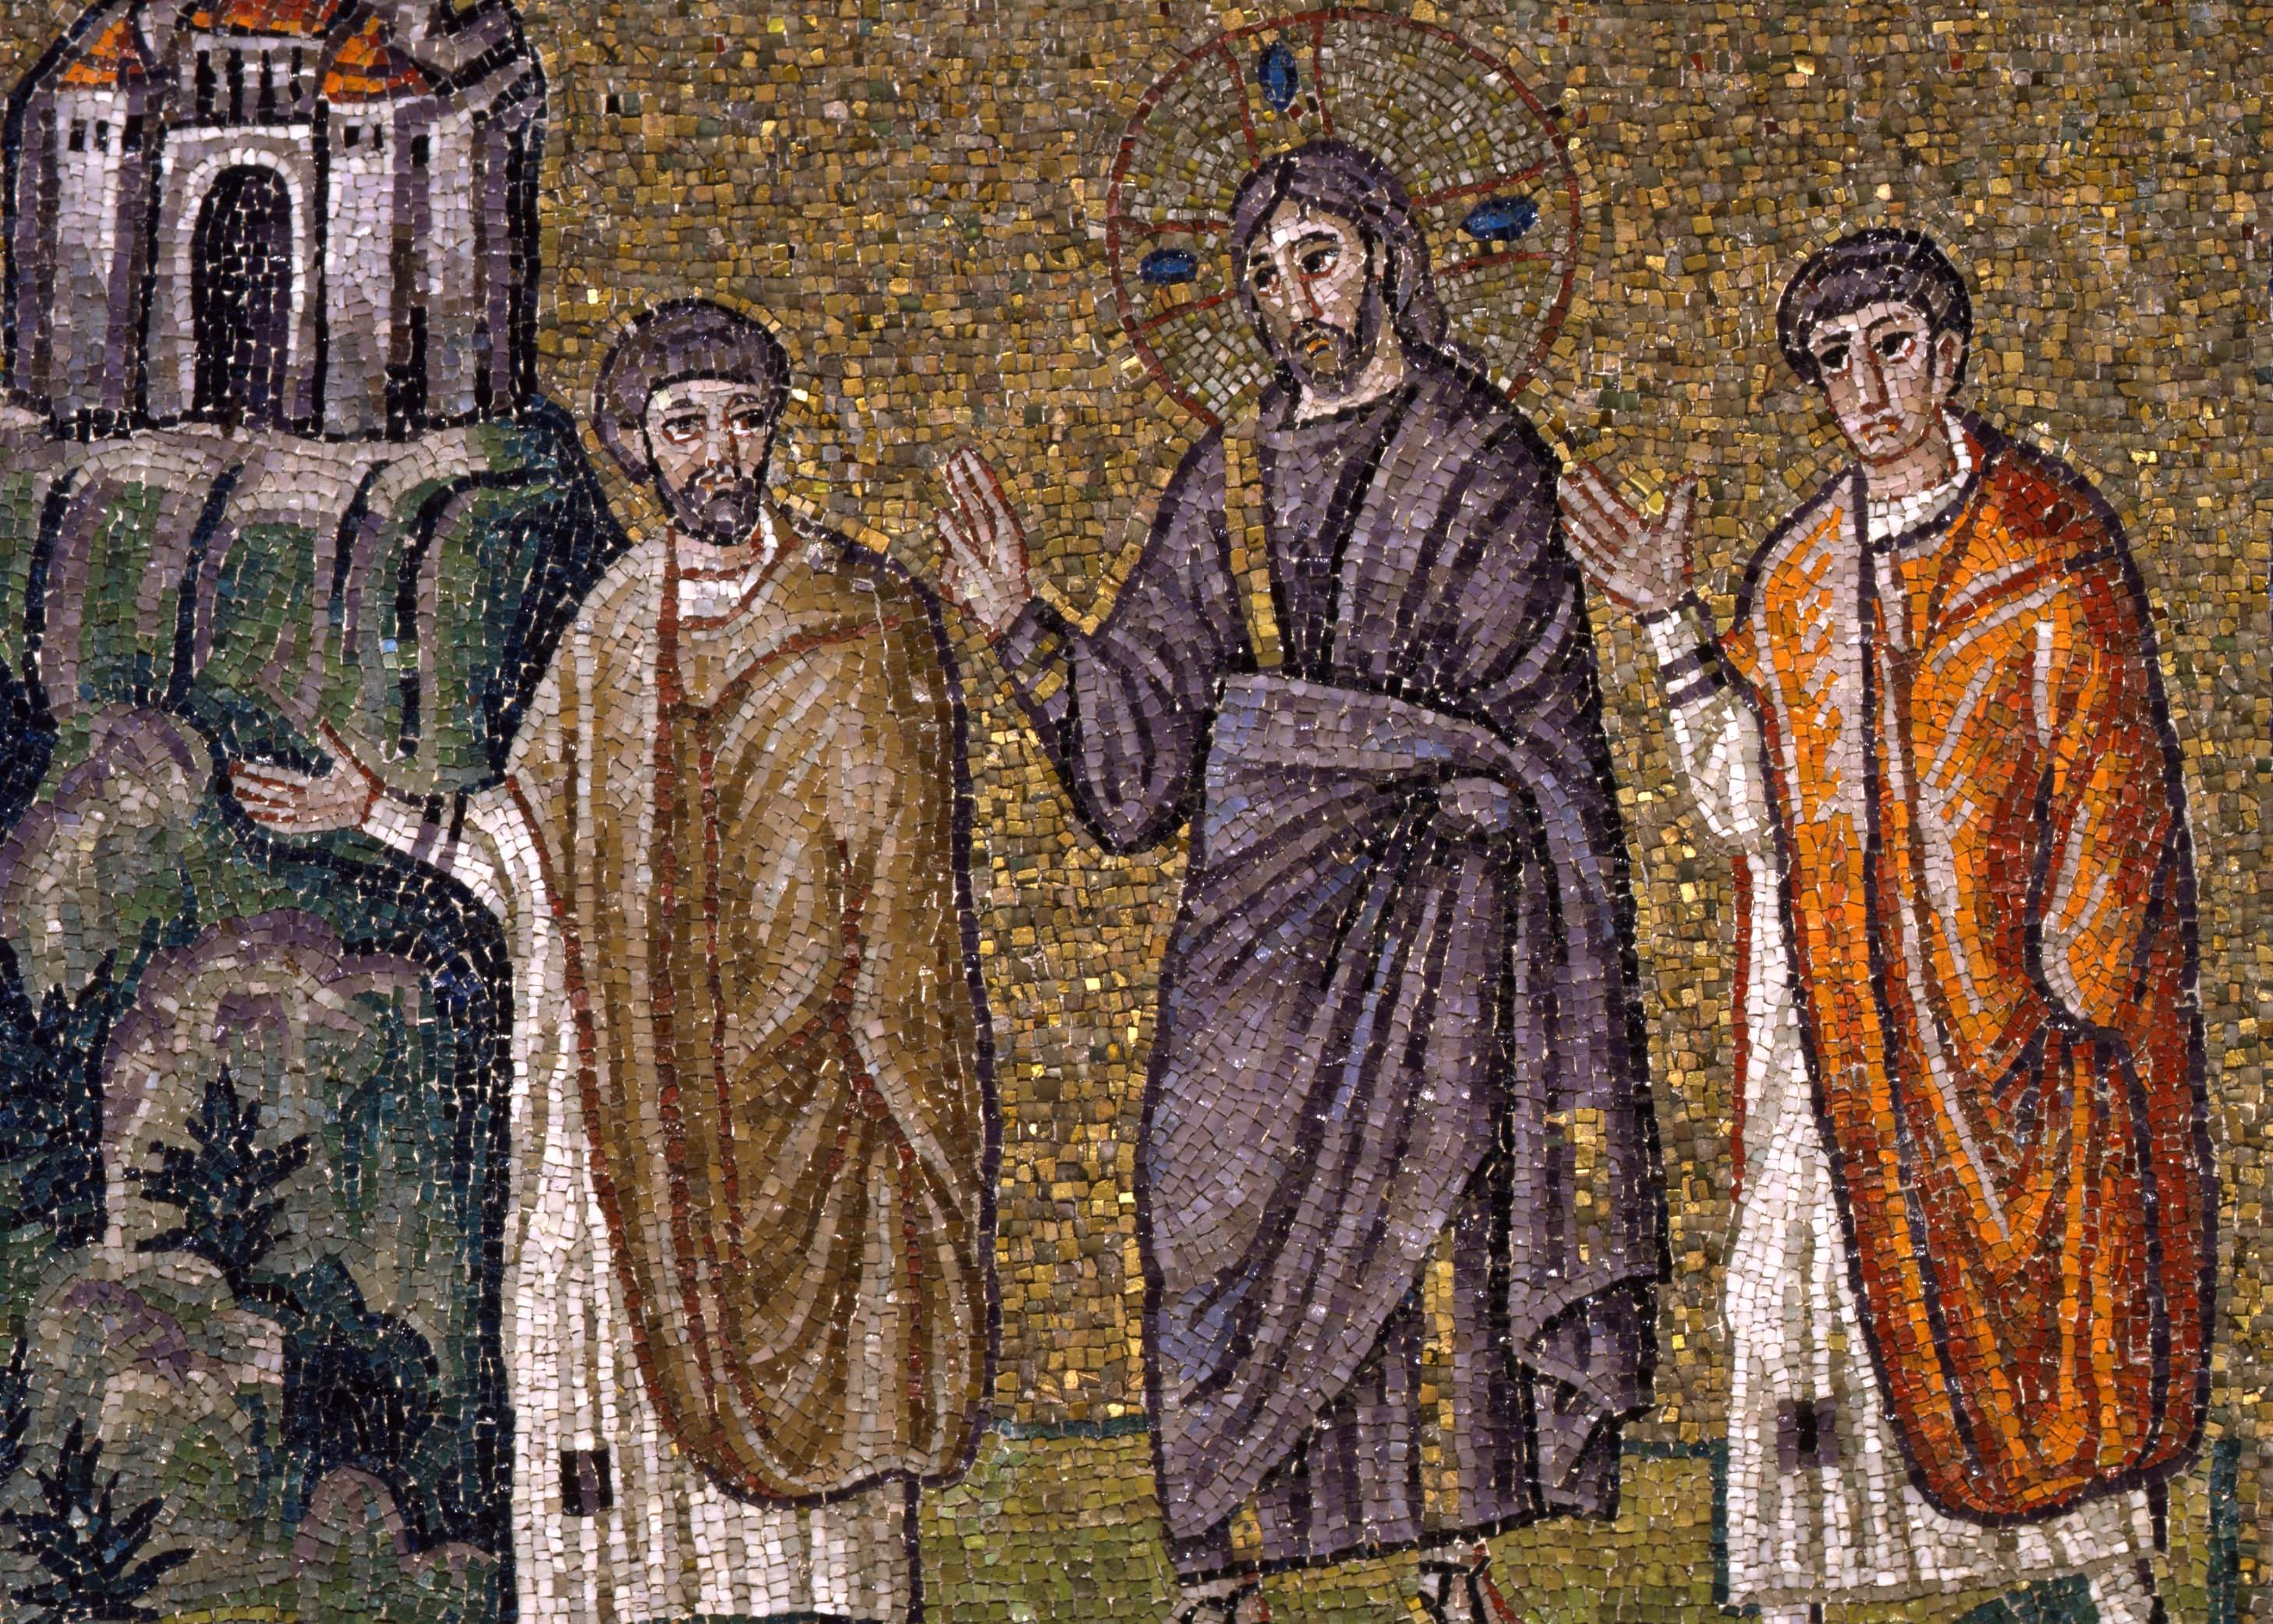
\includegraphics[width=8cm]{emmaus.jpg}
%\end{center}

\vfill

\begin{center}
%Ad usum et secundum consuetudines chori \guillemotright{}Conventus Choralis\guillemotleft.

%Editio Sancti Wolfgangi \annusEditionis
\end{center}

\pagebreak

\renewcommand{\headrulewidth}{0pt} % no horiz. rule at the header
\fancyhf{}
\pagestyle{fancy}

\pars{Oratio ante divinum Officium.}

\lettrine{{\color{red}A}}{peri,} Dómine, os meum ad benedicéndum nomen sanctum tuum:
munda quoque cor meum ab ómnibus vanis, pervérsis, et aliénis
cogitatiónibus:
intelléctum illúmina, afféctum inflámma,
ut digne, atténte ac devóte hoc Offícium recitáre váleam,
et exaudíri mérear ante conspéctum Divínæ Maiestátis tuæ.
Per Christum, Dóminum nostrum.
\Rbardot{} Amen.

Dómine, in unióne illíus divínæ intentiónis,
qua ipse in terris laudes Deo persolvísti,
has tibi Horas \rubricatum{(vel \textnormal{hanc tibi Horam})} persólvo.

%\trOratioAnteOfficium

\vfill

\pars{Oratio post divinum Officium.}

\rubrica{
  Orationem sequentem devote post Officium recitantibus
  Leo Papa X. defectus, et culpas in eo persolvendo ex humana
  fragilitate contractas, indulsit, et dicitur flexis genibus.
}

\lettrine{{\color{red}S}}{acrosánctæ} et indivíduæ Trinitáti,
crucifíxi Dómini nostri Iesu Christi humanitáti,
beatíssimæ et gloriosíssimæ sempérque Vírginis Maríæ
fecúndæ integritáti, 
et ómnium Sanctórum universitáti
sit sempitérna laus, honor, virtus et glória
ab omni creatúra,
nobísque remíssio ómnium peccatórum,
per infiníta sǽcula sæculórum.
\Rbardot{} Amen.

\noindent \Vbardot{} Beáta víscera Maríæ Virginis, quæ portavérunt
ætérni Patris Fílium.\\
\Rbardot{} Et beáta úbera, quæ lactavérunt Christum Dominum.

\rubrica{Et dicitur secreto \textnormal{Pater noster.} et \textnormal{Ave María.}}

%\trOratioPostOfficium

\vfill

\hora{Ad I. Vesperas.} %%%%%%%%%%%%%%%%%%%%%%%%%%%%%%%%%%%%%%%%%%%%%%%%%%%%%
%\sideThumbs{I. Vesperæ}

\cantusSineNeumas

\vspace{0.5cm}
\grechangedim{interwordspacetext}{0.18 cm plus 0.15 cm minus 0.05 cm}{scalable}%
\cuminitiali{}{temporalia/deusinadiutorium-solemnis.gtex}
\grechangedim{interwordspacetext}{0.22 cm plus 0.15 cm minus 0.05 cm}{scalable}%

\vfill
\pagebreak

\pars{Psalmus 1.}

\vspace{-0.4cm}

\antiphona{VII c\textsuperscript{2}}{temporalia/ant-alleluia1.gtex}

\scriptura{Psalmus 144, 10-21.}

\initiumpsalmi{temporalia/ps144ii-initium-vii-c2-auto.gtex}

%\psalmusEtTranslatioT{temporalia/ps144ii-comb.tex}{10cm}
\input{temporalia/ps144ii.tex}

\vspace{-1cm}

\vfill
\pagebreak

\pars{Psalmus 2.}

\scriptura{Psalmus 145.}

\initiumpsalmi{temporalia/ps145-initium-vii-c2-auto.gtex}

%\psalmusEtTranslatioT{temporalia/ps145-comb.tex}{10cm}
\input{temporalia/ps145.tex}

\vfill
\pagebreak

\pars{Psalmus 3.}

\scriptura{Psalmus 146.}

\initiumpsalmi{temporalia/ps146-initium-vii-c2-auto.gtex}

%\psalmusEtTranslatioT{temporalia/ps146-comb.tex}{10cm}
\input{temporalia/ps146.tex}

\vfill
\pagebreak

\pars{Psalmus 4.}

\scriptura{Psalmus 147.}

\initiumpsalmi{temporalia/ps147-initium-vii-c2-auto.gtex}

%\psalmusEtTranslatioT{temporalia/ps147-comb.tex}{10cm}
\input{temporalia/ps147.tex}

\vfill

\vspace{-6mm}

\antiphona{}{temporalia/ant-alleluia1.gtex} % repeat the antiphon - new page

\vfill
\pagebreak

\capitulumLaudes

% preklad Jeruz. bible
%\trCapituliI

\vfill

\pars{Responsorium breve.} \scriptura{Lc. 24, 34}

\cuminitiali{VI}{temporalia/respbr-vesp.gtex}

%\trResp

\vfill
\pagebreak

\pars{Hymnus}

\cuminitiali{VIII}{temporalia/hym-AdCoenam.gtex}
\vspace{-3mm}
%\begin{translatioMulticol}{4}
U~Beránkovy hostiny\\
oděni rouchy bílými,\\
když Rudým mořem prošli jsme,\\
Vladaři Kristu zpívejme.\\
\\
Když jeho tělem posvátným,\\
na kříži obětovaným,\\
se sytíme a~pijeme\\
jeho krev, v~Bohu žijeme.\columnbreak

Chráněni tímto pokrmem\\
před smrtonosným andělem,\\
svrhli jsme z~beder kruté jho\\
tyrana bezohledného.\\
\\
Kristus je naší paschou teď,\\
on sám se vydal za oběť\\
a~místo přesnic našim rtům\\
své tělo dává za pokrm.\columnbreak

Tys, nejčistější Oběti,\\
zlomila vládu podsvětí.\\
Z~otroctví lid je vykoupen,\\
odměna žití kyne všem.\\
\\
Hle, Kristus, když vstal ze hrobu,\\
jde z~pekel v~slavném průvodu\\
a~brány nebes otevřev,\\
vládce tmy vleče v~okovech.\columnbreak

Buď věčně, Kriste, věrným svým\\
plesáním velikonočním.\\
Nás, milostí tvou vzkříšené,\\
vem k~oslavě své vítězné. \\
\\
Sláva tobě, Pane,\\
jenž jsi vstal z~mrtvých,\\
s~Otcem i~Svatým Duchem\\
na věčné věky.\\
Amen.
\end{translatioMulticol}


\vfill
\pagebreak

\pars{Versus.} \scriptura{Lc. 24, 29}

% Versus. %%%
\sineinitiali{temporalia/versus-mane.gtex}

%\noindent \trVersus

\vfill
\pagebreak

\magnificati

\vspace{-1cm}

\vfill
\pagebreak

%\sideThumbs{{\scriptsize{}Fine horarum}}

\anteOrationem

\pagebreak

% Oratio. %%%
\oratioLaudes

\vspace{-1mm}
%\trOrationisI

\vfill

\rubrica{Hebdomadarius dicit iterum Dominus vobiscum. Postea cantatur a cantore:}
\vspace{2mm}

\cuminitiali{VII}{temporalia/benedicamus-tempore-paschali.gtex}

\vspace{1mm}

\vfill
\pagebreak

\hora{Ad Matutinum.} %%%%%%%%%%%%%%%%%%%%%%%%%%%%%%%%%%%%%%%%%%%%%%%%%%%%%
%\sideThumbs{Matutinum}

\vspace{2mm}

\cuminitiali{}{temporalia/dominelabiamea.gtex}

\vspace{2mm}

\pars{Invitatorium.} \scriptura{Lc. 24, 34; Psalmus 94; \textbf{H232}}

\vspace{-6mm}

\antiphona{VI}{temporalia/inv-surrexitdominusvere.gtex}

\vfill
\pagebreak

\pars{Hymnus.}

\vspace{-5mm}

\scriptura{\textbf{AR454}}

{
\grechangedim{interwordspacetext}{0.30 cm plus 0.15 cm minus 0.05 cm}{scalable}%
\antiphona{IV}{temporalia/hym-RexSempiterne.gtex}
\grechangedim{interwordspacetext}{0.32 cm plus 0.15 cm minus 0.05 cm}{scalable}%
}
%{
%\vspace{-5mm}
%\setlength{\columnsep}{0pt} % prostor mezi sloupci
%\input{hym-RexSempiterne-bohtext.tex}
%\setlength{\columnsep}{30pt} % prostor mezi sloupci
%}

\vfill
\pagebreak

\subhora{In I. Nocturno}

\pars{Psalmus 1.} \scriptura{\textbf{H230}}

%\vspace{-5mm}

\antiphona{V a}{temporalia/ant-alleluialapis.gtex}

%\vspace{-5mm}

\scriptura{Ps. 1}

%\vspace{-2mm}

\initiumpsalmi{temporalia/ps1-initium-v-a-auto.gtex}

%\psalmusEtTranslatioT{temporalia/ps1-comb.tex}{10cm}

\input{temporalia/ps1.tex}

\vfill
\pagebreak

\pars{Psalmus 2.}

\scriptura{Ps. 2}

\initiumpsalmi{temporalia/ps2-initium-v-a-auto.gtex}

%\psalmusEtTranslatioT{temporalia/ps2-comb.tex}{10cm}

\input{temporalia/ps2.tex}

\vfill
\pagebreak

\pars{Psalmus 3.}

\scriptura{Ps. 3}

\initiumpsalmi{temporalia/ps3-initium-v-a-auto.gtex}

%\psalmusEtTranslatioT{temporalia/ps3-comb.tex}{10cm}

\input{temporalia/ps3.tex}

\vfill

\antiphona{}{temporalia/ant-alleluialapis.gtex}

\vfill
\pagebreak

\noindent \Vbardot{} Surréxit Dóminus de sepúlcro, allelúia.
\noindent \Rbardot{} Qui pro nobis pepéndit in ligno, allelúia.

\noindent Pater noster.

\pars{Absolutio.}

\cuminitiali{}{temporalia/absolutio-exaudi.gtex}

\vfill
\pagebreak

\cuminitiali{}{temporalia/benedictio-solemn-benedictione.gtex}

\vspace{7mm}

\lectioi

\noindent \Vbardot{} Tu autem, Dómine, miserére nobis.
\noindent \Rbardot{} Deo grátias.

\vfill
\pagebreak

\responsoriumi

\vfill
\pagebreak

\cuminitiali{}{temporalia/benedictio-solemn-unigenitus.gtex}

\vspace{7mm}

\lectioii

\noindent \Vbardot{} Tu autem, Dómine, miserére nobis.
\noindent \Rbardot{} Deo grátias.

\vfill
\pagebreak

\responsoriumii

\vfill
\pagebreak

\cuminitiali{}{temporalia/benedictio-solemn-spiritus.gtex}

\vspace{7mm}

\lectioiii

\noindent \Vbardot{} Tu autem, Dómine, miserére nobis.
\noindent \Rbardot{} Deo grátias.

\vfill
\pagebreak

\responsoriumiii

\vfill
\pagebreak

\subhora{In II. Nocturno}

\pars{Psalmus 4.} \scriptura{Io. 20, 15; \textbf{H241}}

%\vspace{-5mm}

\antiphona{V a}{temporalia/ant-alleluiaquem.gtex}

%\vspace{-5mm}

\scriptura{Ps. 8}

%A\vspace{-2mm}

\initiumpsalmi{temporalia/ps8-initium-v-a-auto.gtex}

%\psalmusEtTranslatioT{temporalia/ps8-comb.tex}{10cm}

\input{temporalia/ps8.tex}

\vfill
\pagebreak

\pars{Psalmus 5.}

\scriptura{Ps. 9, 2-11}

\initiumpsalmi{temporalia/ps9ii_xi-initium-v-a-auto.gtex}

%\psalmusEtTranslatioT{temporalia/ps9ii_xi-comb.tex}{10cm}

\input{temporalia/ps9ii_xi.tex}

\vfill
\pagebreak

\pars{Psalmus 6.}

\scriptura{Ps. 9, 12-21}

\initiumpsalmi{temporalia/ps9xii_xxi-initium-v-a-auto.gtex}

%\psalmusEtTranslatioT{temporalia/ps9xii_xxi-comb.tex}{10cm}

\input{temporalia/ps9xii_xxi.tex}

\vfill

\antiphona{}{temporalia/ant-alleluiaquem.gtex}

\vfill
\pagebreak

\noindent \Vbardot{} Surréxit Dóminus vere, allelúia.
\noindent \Rbardot{} Et appáruit Simóni, allelúia.

\noindent Pater noster.

\pars{Absolutio.}

\cuminitiali{}{temporalia/absolutio-ipsius.gtex}

\vfill
\pagebreak

\cuminitiali{}{temporalia/benedictio-solemn-deus.gtex}

\vspace{7mm}

\lectioiv

\noindent \Vbardot{} Tu autem, Dómine, miserére nobis.
\noindent \Rbardot{} Deo grátias.

\vfill
\pagebreak

\responsoriumiv

\vfill
\pagebreak

\cuminitiali{}{temporalia/benedictio-solemn-christus.gtex}

\vspace{7mm}

\lectiov

\noindent \Vbardot{} Tu autem, Dómine, miserére nobis.
\noindent \Rbardot{} Deo grátias.

\vfill
\pagebreak

\responsoriumv

\vfill
\pagebreak

\cuminitiali{}{temporalia/benedictio-solemn-ignem.gtex}

\vspace{7mm}

\lectiovi

\noindent \Vbardot{} Tu autem, Dómine, miserére nobis.
\noindent \Rbardot{} Deo grátias.

\vfill
\pagebreak

\responsoriumvi

\vfill
\pagebreak

\subhora{In III. Nocturno}

\pars{Psalmus 7.} \scriptura{Cf. Io. 20, 15; \textbf{H241}}

\vspace{-5mm}

\antiphona{V a}{temporalia/ant-alleluianoli.gtex}

\vspace{-4mm}

\scriptura{Ps. 9, 22-32}

%\vspace{-2mm}

\initiumpsalmi{temporalia/ps9xxii_xxxii-initium-v-a-auto.gtex}

%\psalmusEtTranslatioT{temporalia/ps9xxii_xxxii-comb.tex}{10cm}

\input{temporalia/ps9xxii_xxxii.tex}

\vfill
\pagebreak

\pars{Psalmus 8.}

\scriptura{Ps. 9, 33-39}

\initiumpsalmi{temporalia/ps9xxxiii_xxxix-initium-v-a-auto.gtex}

%\psalmusEtTranslatioT{temporalia/ps9xxxiii_xxxix-comb.tex}{10cm}

\input{temporalia/ps9xxxiii_xxxix.tex}

\vfill
\pagebreak

\pars{Psalmus 9.}

\scriptura{Ps. 10}

\initiumpsalmi{temporalia/ps10-initium-v-a-auto.gtex}

%\psalmusEtTranslatioT{temporalia/ps10-comb.tex}{10cm}

\input{temporalia/ps10.tex}

\vfill

\antiphona{}{temporalia/ant-alleluianoli.gtex}

\vfill
\pagebreak

\noindent \Vbardot{} Gavísi sunt discípuli, allelúia.
\noindent \Rbardot{} Viso Dómino, allelúia.

\noindent Pater noster.

\pars{Absolutio.}

\cuminitiali{}{temporalia/absolutio-avinculis.gtex}

\vfill
\pagebreak

\cuminitiali{}{temporalia/benedictio-solemn-evangelica.gtex}

\vspace{7mm}

\lectiovii

\noindent \Vbardot{} Tu autem, Dómine, miserére nobis.
\noindent \Rbardot{} Deo grátias.

\vfill
\pagebreak

\responsoriumvii

\vfill
\pagebreak

\cuminitiali{}{temporalia/benedictio-solemn-divinum.gtex}

\vspace{7mm}

\lectioviii

\noindent \Vbardot{} Tu autem, Dómine, miserére nobis.
\noindent \Rbardot{} Deo grátias.

\vfill
\pagebreak

\responsoriumviii

\vfill
\pagebreak

\cuminitiali{}{temporalia/benedictio-solemn-adsocietatem.gtex}

\vspace{7mm}

\lectioix

\noindent \Vbardot{} Tu autem, Dómine, miserére nobis.
\noindent \Rbardot{} Deo grátias.

\vfill
\pagebreak

% Te Deum

%\pars{Hymnus Ambrosianus}

\vspace{-5mm}

{
\grechangedim{interwordspacetext}{0.22 cm plus 0.15 cm minus 0.05 cm}{scalable}%
\cuminitiali{III}{temporalia/tedeum-solemnis.gtex}
\grechangedim{interwordspacetext}{0.32 cm plus 0.15 cm minus 0.05 cm}{scalable}%
}

\vfill
\pagebreak

\rubrica{Reliqua omittuntur, nisi Laudes separandæ sint.}

\pars{Oratio}

\noindent \Vbardot{} Dómine, exáudi oratiónem meam.

\noindent \Rbardot{} Et clamor meus ad te véniat.

Orémus:

\oratioMatutinum

\noindent \Rbardot{} Amen.

\vspace{7mm}

\pars{Conclusio}

\noindent \Vbardot{} Dómine, exáudi oratiónem meam.

\noindent \Rbardot{} Et clamor meus ad te véniat.

\noindent \Vbardot{} Benedicámus Dómino, allelúia, allelúia.

\noindent \Rbardot{} Deo grátias, allelúia, allelúia.

\noindent \Vbardot{} Fidélium ánimæ per misericórdiam Dei requiéscant in pace.

\noindent \Rbardot{} Amen.

\vfill
\pagebreak

\hora{Ad Laudes.} %%%%%%%%%%%%%%%%%%%%%%%%%%%%%%%%%%%%%%%%%%%%%%%%%%%%%
%\sideThumbs{Laudes}

\cantusSineNeumas

\vspace{0.5cm}
\grechangedim{interwordspacetext}{0.18 cm plus 0.15 cm minus 0.05 cm}{scalable}%
\cuminitiali{}{temporalia/deusinadiutorium-alter.gtex}
\grechangedim{interwordspacetext}{0.22 cm plus 0.15 cm minus 0.05 cm}{scalable}%

\vfill
%\pagebreak

\pars{Psalmus 1.}

\vspace{-0.4cm}

\antiphona{VIII G}{temporalia/ant-alleluia2.gtex}

\scriptura{Psalmus 92.}

\initiumpsalmi{temporalia/ps92-initium-viii-g-auto.gtex}

%\psalmusEtTranslatioT{temporalia/ps92-comb.tex}{10cm}
\input{temporalia/ps92.tex}

\vspace{-1cm}

\vfill
\pagebreak

\pars{Psalmus 2.}

\scriptura{Psalmus 99.}

\initiumpsalmi{temporalia/ps99-initium-viii-g-auto.gtex}

%\psalmusEtTranslatioT{temporalia/ps99-comb.tex}{10cm}
\input{temporalia/ps99.tex}

\vfill
\pagebreak

\pars{Psalmus 3.}

\scriptura{Psalmus 62.}

\initiumpsalmi{temporalia/ps62-initium-viii-g-auto.gtex}

%\psalmusEtTranslatioT{temporalia/ps62-comb.tex}{10cm}
\input{temporalia/ps62.tex}

\vfill

\vspace{-6mm}

\antiphona{}{temporalia/ant-alleluia2.gtex} % repeat the antiphon - new page

\vfill
\pagebreak

\pars{Psalmus 4.}

\vspace{-0.4cm}

\antiphona{VI F}{temporalia/ant-surrexitchristus.gtex}

\scriptura{Canticum trium puerorum, Dan. 3, 57-88 et 56}

\initiumpsalmi{temporalia/dan3-initium-vi-F-auto.gtex}

%\psalmusEtTranslatioT{temporalia/dan3-comb.tex}{10cm}
\input{temporalia/dan3.tex}

\vfill

\vspace{-6mm}

\antiphona{}{temporalia/ant-surrexitchristus.gtex} % repeat the antiphon - new page

\vfill
\pagebreak

\pars{Psalmus 5.}

\vspace{-0.4cm}

\antiphona{VI F}{temporalia/ant-alleluia3.gtex}

\scriptura{Psalmus 148.}

\initiumpsalmi{temporalia/ps148-initium-vi-F-auto.gtex}

%\psalmusEtTranslatioT{temporalia/ps148-comb.tex}{10cm}
\input{temporalia/ps148.tex}

\rubrica{Hic non dicitur Gloria Patri.}

\vfill
\pagebreak

%
\scriptura{Psalmus 149.}

\initiumpsalmi{temporalia/ps149-initium-vi-F-auto.gtex}

%\psalmusEtTranslatioT{temporalia/ps149-comb.tex}{10cm}
\input{temporalia/ps149.tex}

\rubrica{Hic non dicitur Gloria Patri.}

\vfill
\pagebreak

%
\scriptura{Psalmus 150.}

\initiumpsalmi{temporalia/ps150-initium-vi-F-auto.gtex}

%\psalmusEtTranslatioT{temporalia/ps150-comb.tex}{10cm}
\input{temporalia/ps150.tex}

\vfill

\vspace{-6mm}

\antiphona{}{temporalia/ant-alleluia3.gtex} % repeat the antiphon - new page

\vfill
\pagebreak

\capitulumLaudes

% preklad Jeruz. bible
%\trCapituliI

\vfill

\pars{Responsorium breve.} \scriptura{Cf. Mt. 28, 6; Cf. Gal. 3, 13}

\cuminitiali{VI}{temporalia/respbr-laud.gtex}

%\trResp

\vfill
\pagebreak

\pars{Hymnus}

\cuminitiali{VIII}{temporalia/hym-AuroraLucis.gtex}
\vspace{-3mm}
%\input{hym-AuroraLucis-bohtext.tex}

\vfill
%\pagebreak

\pars{Versus.}

% Versus. %%%
\sineinitiali{temporalia/versus-inresurrectione.gtex}

%\noindent \trVersus

\vfill
\pagebreak

\benedictus

\vspace{-1cm}

\vfill
\pagebreak

%\sideThumbs{{\scriptsize{}Fine horarum}}

\anteOrationem

\pagebreak

% Oratio. %%%
\oratioLaudes

\vspace{-1mm}
%\trOrationisI

\vfill

\rubrica{Hebdomadarius dicit iterum Dominus vobiscum. Postea cantatur a cantore:}
\vspace{2mm}

\cuminitiali{VII}{temporalia/benedicamus-tempore-paschali.gtex}

\vspace{1mm}

\vfill
\pagebreak

\hora{Ad II. Vesperas.} %%%%%%%%%%%%%%%%%%%%%%%%%%%%%%%%%%%%%%%%%%%%%%%%%%%%%
%\sideThumbs{II. Vesperæ}

\cantusSineNeumas

\vspace{0.5cm}
\grechangedim{interwordspacetext}{0.18 cm plus 0.15 cm minus 0.05 cm}{scalable}%
\cuminitiali{}{temporalia/deusinadiutorium-solemnis.gtex}
\grechangedim{interwordspacetext}{0.22 cm plus 0.15 cm minus 0.05 cm}{scalable}%

\vfill
%\pagebreak

\vspace{-2mm}

\pars{Psalmus 1.}

\vspace{-0.4cm}

\antiphona{VII c\textsuperscript{2}}{temporalia/ant-alleluia4.gtex}

\vspace{-4mm}

\scriptura{Psalmus 109.}

\initiumpsalmi{temporalia/ps109-initium-vii-c2-auto.gtex}

%\psalmusEtTranslatioT{temporalia/ps109-comb.tex}{10cm}
\input{temporalia/ps109.tex}

\vspace{-1cm}

\vfill
\pagebreak

\pars{Psalmus 2.}

\scriptura{Psalmus 110.}

\initiumpsalmi{temporalia/ps110-initium-vii-c2-auto.gtex}

%\psalmusEtTranslatioT{temporalia/ps110-comb.tex}{10cm}
\input{temporalia/ps110.tex}

\vfill
\pagebreak

\pars{Psalmus 3.}

\scriptura{Psalmus 111.}

\initiumpsalmi{temporalia/ps111-initium-vii-c2-auto.gtex}

%\psalmusEtTranslatioT{temporalia/ps111-comb.tex}{10cm}
\input{temporalia/ps111.tex}

\vfill
\pagebreak

\pars{Psalmus 4.}

\scriptura{Psalmus 112.}

\initiumpsalmi{temporalia/ps112-initium-vii-c2-auto.gtex}

%\psalmusEtTranslatioT{temporalia/ps112-comb.tex}{10cm}
\input{temporalia/ps112.tex}

\vfill

\vspace{-6mm}

\antiphona{}{temporalia/ant-alleluia4.gtex} % repeat the antiphon - new page

\vfill
\pagebreak

\capitulumLaudes

% preklad Jeruz. bible
%\trCapituliI

\vfill

\pars{Responsorium breve.} \scriptura{Lc. 24, 34}

\cuminitiali{VI}{temporalia/respbr-vesp.gtex}

%\trResp

\vfill
\pagebreak

\pars{Hymnus}

\cuminitiali{VIII}{temporalia/hym-AdCoenam.gtex}
\vspace{-3mm}
%\begin{translatioMulticol}{4}
U~Beránkovy hostiny\\
oděni rouchy bílými,\\
když Rudým mořem prošli jsme,\\
Vladaři Kristu zpívejme.\\
\\
Když jeho tělem posvátným,\\
na kříži obětovaným,\\
se sytíme a~pijeme\\
jeho krev, v~Bohu žijeme.\columnbreak

Chráněni tímto pokrmem\\
před smrtonosným andělem,\\
svrhli jsme z~beder kruté jho\\
tyrana bezohledného.\\
\\
Kristus je naší paschou teď,\\
on sám se vydal za oběť\\
a~místo přesnic našim rtům\\
své tělo dává za pokrm.\columnbreak

Tys, nejčistější Oběti,\\
zlomila vládu podsvětí.\\
Z~otroctví lid je vykoupen,\\
odměna žití kyne všem.\\
\\
Hle, Kristus, když vstal ze hrobu,\\
jde z~pekel v~slavném průvodu\\
a~brány nebes otevřev,\\
vládce tmy vleče v~okovech.\columnbreak

Buď věčně, Kriste, věrným svým\\
plesáním velikonočním.\\
Nás, milostí tvou vzkříšené,\\
vem k~oslavě své vítězné. \\
\\
Sláva tobě, Pane,\\
jenž jsi vstal z~mrtvých,\\
s~Otcem i~Svatým Duchem\\
na věčné věky.\\
Amen.
\end{translatioMulticol}


\vfill
\pagebreak

\pars{Versus.} \scriptura{Lc. 24, 29}

% Versus. %%%
\sineinitiali{temporalia/versus-mane.gtex}

%\noindent \trVersus

\vfill
\pagebreak

\magnificatii

\vspace{-1cm}

\vfill
\pagebreak

%\sideThumbs{{\scriptsize{}Fine horarum}}

\anteOrationem

\pagebreak

% Oratio. %%%
\oratioLaudes

\vspace{-1mm}
%\trOrationisI

\vfill

\rubrica{Hebdomadarius dicit iterum Dominus vobiscum. Postea cantatur a cantore:}
\vspace{2mm}

\cuminitiali{VII}{temporalia/benedicamus-tempore-paschali.gtex}

\vspace{1mm}

\newpage
\RemoveSideThumbs
\pagestyle{empty}

\pars{Antiphona finalis B. M. V. pro Tempore Paschali.}

\cuminitiali{VI}{temporalia/an_regina_caeli_simplex.gtex}
%\trReginaCaeli

%%% COLOPHON
%\vfill

%Fontes.
%Textus et cantus officii divini secundum
%Antiphonale Sacrosanctæ Romanæ Eclesiæ Pro Diurnis Horis, Romæ 1912, præter:
%hymni et responsoria breve secundum Antiphonale Monasticum pro Diurnis Horis,
%Solesmis 1934. /
%Translatio capituli sumpta est ex: Jeruzalémská bible, Praha-Kostelní Vydří 2009. /
%Translationes psalmorum ex Hejčl Jan: Žaltář čili Kniha žalmů, Praha 1922. /
%Neumæ super canto officii divini de codice Hartker, Stiftsbibl. 391.

%Collaborantes.
%Textus latinos cantusque transcripsit et omnem laborem typographicum peregit
%Jakub Jelínek. /
%Psalmos in lingua bohemica de libro transcripserunt Barbora Maturová et idem Jakub Jelínek. /
%Václav Ondráček textus responsoriorum in linguam bohemicam transtulit. /
%Mons. Jiří Reinsberg \olddag{} et Jana Kuběnová textus deprecationum in linguam bohemicam transtulerunt. /
%Zbyněk Šír et Filip Srovnal librum istum præparare mandaverunt et laborem exprobrationibus
%utilissimis comitabantur.

%Instrumenta adhibita.
%LuaTeX, %http://www.luatex.org /
%Gregorio, %http://home.gna.org/gregorio /
%typi Junicode. %http://junicode.sourceforge.net

%\begin{center}
%Liber hic imprimis ad usum chori
%\guillemotright Conventus Choralis\guillemotleft\
%paratus est
%et secundum eius consuetudines.
%http://www.introitus.cz

%\vfill

%{\large Editio Sancti Wolfgangi \annusEditionis.}

%\vfill

%Series \guillemotright Conventus\guillemotleft, vol. X.

%\vfill

%http://stiwolfgangi.xf.cz

%\vfill

%\today

%\end{center}

\end{document}

